\section{Experiment 2: Three-Round Architecture Audit}
\label{sec:exp2}

\subsection{Design}
Three rounds, each with a distinct epistemic function:
\begin{enumerate}\setlength{\itemsep}{0pt}\setlength{\parskip}{0pt}\setlength{\parsep}{0pt}
\item \textbf{Round 1 (component-wise adjudication).} 21 engine components enumerated; each adjudicated against the state of the art.
\item \textbf{Round 2 (independent re-review).} 47 claims re-examined by a second reviewer; 30 REVISE / 5 REPLACE, overturning several prior numbers. ``Independent'' here means independent \emph{within the audit pipeline} (a separate reviewer persona executing against a frozen evidence set, with no access to the prior round's conclusions until after independent adjudication); it does not mean external review by third-party scholars, and we do not claim that.
\item \textbf{Round 3 (literature + adversarial).} Six literature lanes (arXiv/Crossref/ERIC) plus three red-team attack passes plus one independent verification round.
\end{enumerate}

\subsection{Quantified findings}

Figure~\ref{fig:auditnums} plots the measurements that survived re-verification.

\begin{figure}[t]
\centering
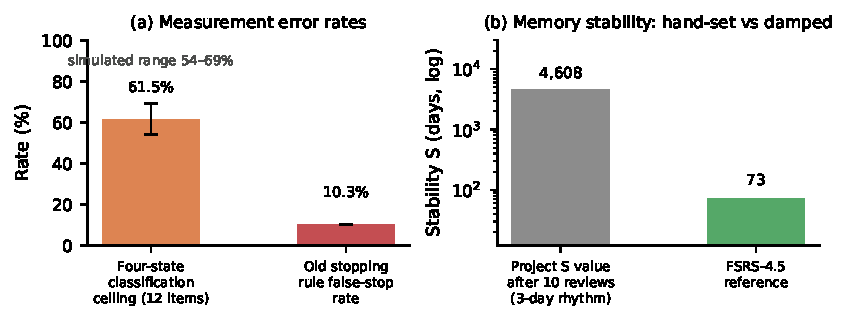
\includegraphics[width=\textwidth]{figures/fig5_audit_numbers.pdf}
\caption{The hardest audit numbers. (a) Measurement error rates with simulation range; (b) memory stability: the hand-set formula produced S=4,608~d vs.\ the FSRS-4.5 reference of 73~d after 10 reviews at a 3-day rhythm.}
\label{fig:auditnums}
\end{figure}

\begin{table}[h]
\centering
\small
\begin{tabular}{@{}p{6.4cm}p{3.2cm}p{4.0cm}@{}}
\toprule
\textbf{Finding} & \textbf{Value} & \textbf{Source} \\
\midrule
Four-state classification accuracy after 12 items & 54--69\% (two sim. runs) & redteam 1 \\
P/U non-identifiability & KL = 0.0247 & lane 1; redteam 1 \\
Old stopping (gap $>$ 0.45) false-stop & 10.3\% & redteam 1 \\
FSRS hand-set multipliers, 10 reviews & S = 4,608 d (4.5: 73) & redteam 2; round 4 \\
n=2 held-out one-sided 95\% CI & 22.4\% & round 4 \\
SymPy \texttt{simplify} false equivalences & 7 / 5 reproduced & redteam 3 \\
\bottomrule
\end{tabular}
\caption{The hardest numbers, each traced to the report that produced it. The four-state ceiling is reported as the range across two independent simulation runs (master audit, 2026-08-13); the individual runs in redteam 1 produced 4-way accuracy 61.4\% and 61.1\% at 12 items.}
\label{tab:exp2}
\end{table}

\begin{figure}[t]
\centering
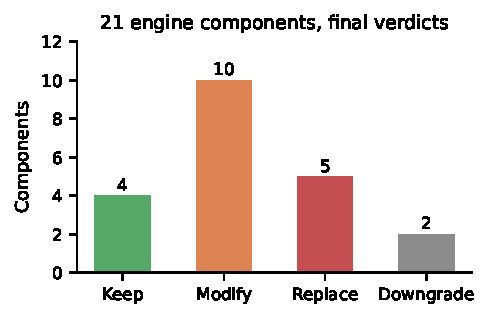
\includegraphics[width=0.55\textwidth]{figures/fig4_audit_verdicts.pdf}
\caption{Final verdicts across the 21 audited engine components.}
\label{fig:verdicts}
\end{figure}
\subsection{Verdicts}
Figure~\ref{fig:verdicts} shows the distribution. Across 21 components: \textbf{4 keep / 10 modify / 5 replace / 2 downgrade} (\texttt{docs/audit-history/MASTER\_AUDIT\_REPORT\_2026-08-13.md}, verified against the frozen evidence matrix of 47 claims: 30 REVISE / 5 REPLACE / 7 EXPERIMENT\_ONLY / 4 UNKNOWN / 1 RETIRE). The final column: inference keeps binary mastery + prerequisite prior + error-code routing (four UI labels retained); stopping becomes P(top1) $\geq$ 0.8 with min\_length 4--5 with gap display-only; memory switches to the FSRS-4.5 damped formula; efficacy score is demoted to a tie-break (5pp real difference at n=20 still flips 30\% of replicates); held-out early-stop protocol becomes 3$\rightarrow$6, never n=2 binary; events gain a provenance field (source $\in$ \{real, qa, synthetic\}).

\subsection{Drop-in changes already in the tree}
Three verdicts are implemented and tested: FSRS-4.5 damped stability with $S_{\max}=500$~d; stopping on P(top1)$\ge$0.80 with min direct answers 4; event provenance with schema\_version 2. Each has regression tests in \texttt{tests/}.

\subsection{What this audit does and does not prove}
It proves that the engine's \emph{design assumptions} are individually checkable, and that three of them were wrong in measurable ways. It does not prove the engine works on students.
